\documentclass{beamer}

\usepackage{minted}
\usepackage{svg}

\usetheme{Boadilla}

\setminted{breaklines}

% Title
\title{Coreutils and The Linux Filesystem}
\subtitle{Linux Week \the\year{}}
\author{Ethan Wong}
\date{\today}
\institute{Linux Users Group @ UIC}

\begin{document}
\begin{frame}
	\titlepage
\end{frame}

\begin{frame}{Table of Contents}
	\tableofcontents[pausesections]
\end{frame}

\section{Filesystem}
\begin{frame}{Why care?}
	\begin{itemize}
		\item Programs, configuration files, temp files, etc. are mostly
			organized by a standard.
			\pause

		\item On *nix-like systems, most interaction with devices can be done
			directly \underline{through the filesystem}.
			\pause

		\item On Linux? Try \texttt{cat /proc/cpuinfo} as an example!
	\end{itemize}
\end{frame}

\begin{frame}{Overview}
	\begin{columns}
		\begin{column}{0.5\textwidth}
			\begin{figure}
				\centering
				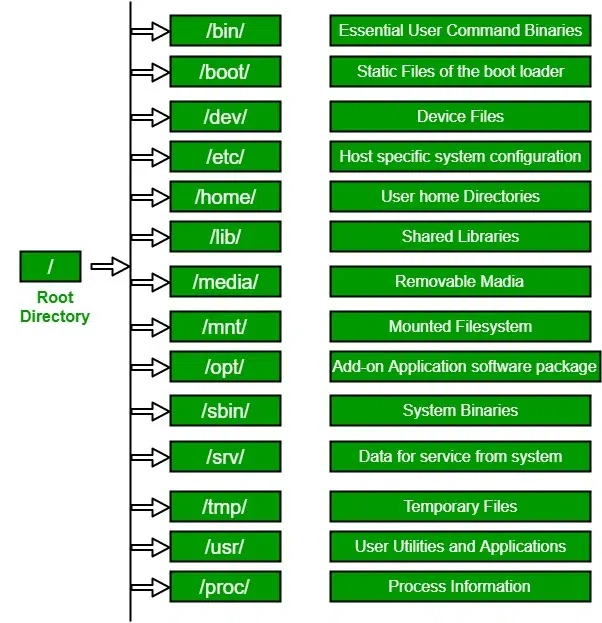
\includegraphics[width=\textwidth]{fhs.png}
			\end{figure}
		\end{column}
		\begin{column}{0.5\textwidth}
			\begin{itemize}
				\item The FS on Linux distros is defined by the Filesystem
					Hierarchy Standard.
					\pause

				\item Does vary slightly depending on distro (some hate
					following standards).
					\pause

				\item Root directory is the parent node of all other
					directories/files on the system.
					\pause

				\item User programs are installed in varying locations within
					the root filesystem.
			\end{itemize}
		\end{column}
	\end{columns}
\end{frame}

\begin{frame}
	\begin{center}
		\Huge How do we interact with the filesystem?
	\end{center}
\end{frame}

\section{Coreutils}
\begin{frame}{Table of Contents}
	\tableofcontents[currentsection]
\end{frame}

\begin{frame}{Intro to Coreutils}
	\begin{center}
		\Huge What are coreutils?
	\end{center}
\end{frame}

\begin{frame}{Common Examples}
	\begin{columns}
		\begin{column}{0.33\textwidth}
			\begin{figure}
				\centering
				\caption{cat}
				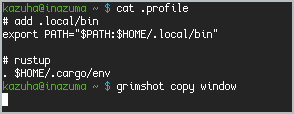
\includegraphics[width=0.7\textwidth]{cat.png}
				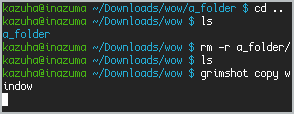
\includegraphics[width=0.7\textwidth]{rm.png}
				\caption{rm}
			\end{figure}
		\end{column}
		\begin{column}{0.33\textwidth}
			\begin{figure}
				\centering
				\caption{ls}
				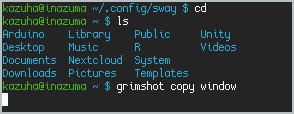
\includegraphics[width=0.7\textwidth]{ls.png}
				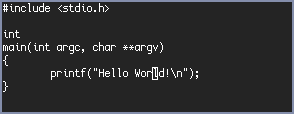
\includegraphics[width=0.7\textwidth]{vi.png}
				\caption{vi}
			\end{figure}
		\end{column}
		\begin{column}{0.33\textwidth}
			\begin{figure}
				\centering
				\caption{mkdir}
				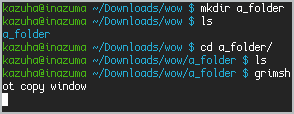
\includegraphics[width=0.7\textwidth]{mkdir.png}
				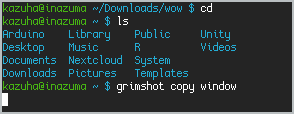
\includegraphics[width=0.7\textwidth]{cd.png}
				\caption{cd}
			\end{figure}
		\end{column}
	\end{columns}
\end{frame}

\begin{frame}{Intro to Coreutils}
	\begin{itemize}
		\item Coreutils are the basic file, shell, and text manipulation
			utlities for a *nix-like operating system.
			\pause

		\item These programs are simple and user-interactable!
			\pause

		\item Defined by a standard called POSIX.
	\end{itemize}
\end{frame}

\begin{frame}{Intro to Coreutils}
	\begin{itemize}
		\item The GNU project was established in 1983 as a free software project
			to build a complete operating system.
			\pause

		\item Nowadays, their version of the POSIX coreutils is the dominant
			implementation used in Linux distributions.
	\end{itemize}
\end{frame}

\begin{frame}{Structure of a Linux Command}
	\begin{Large}
		\textbf{Format} \\
	\end{Large}
	\texttt{\{command\} \{options/flags\} \{arguments\}}

	\vspace{0.3cm}

	\begin{Large}
		\textbf{Example} \\
	\end{Large}
	\texttt{rm -r oldStuff}

	\vspace{0.3cm}

	\begin{tabular}{|c|c|}
		\hline
		Command & \texttt{rm} \\
		\hline
		Flags & \texttt{-r} \\
		\hline
		Arguments & \texttt{oldStuff} \\
		\hline
	\end{tabular}
\end{frame}

\section{Crash Course}
\begin{frame}{Table of Contents}
	\tableofcontents[currentsection]
\end{frame}

\subsection{Terminal and SSH}
\begin{frame}{Crash Course}
	\begin{center}
		\Huge Connecting to a Server
	\end{center}
\end{frame}

\begin{frame}{Connecting to a Server}
	\begin{Large}
		\textbf{Terminal} \\
	\end{Large}
	This is what your computer understands!
	\begin{figure}
		\centering
		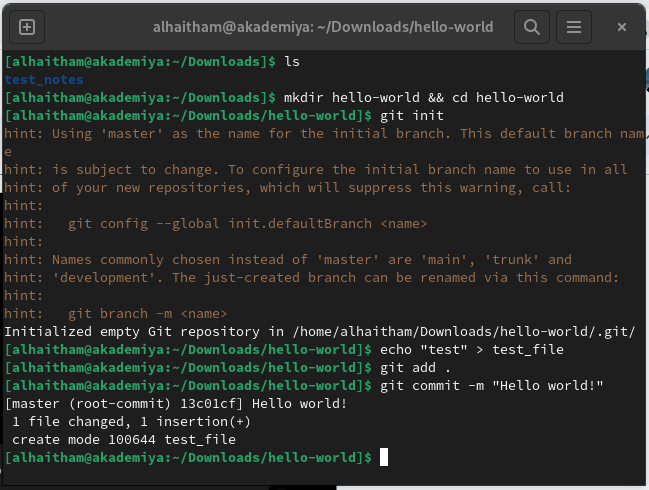
\includegraphics[width=0.5\textwidth]{terminal.png}
		\caption{GNOME Terminal running Bash}
	\end{figure}
\end{frame}

\begin{frame}{Connecting to a Server}
	\begin{Large}
		\textbf{How to get to the terminal?} \\
	\end{Large}
	\begin{tabular}{|c|c|}
		\hline
		Windows & Open \texttt{Windows Powershell} \\
		\hline
		macOS and Linux & Open \texttt{Terminal} \\
		\hline
		iOS & Install \texttt{Terminus} \\
		\hline
		Android & Install \texttt{Termux} and \\
		& \texttt{sudo apt install openssh-client} \\
		\hline
	\end{tabular}
\end{frame}

\begin{frame}
	\begin{center}
		\begin{Huge}
			\texttt{ssh} \\
		\end{Huge}
		OpenSSH SSH client (remote login program)
	\end{center}
\end{frame}

\begin{frame}{SSH}
	\begin{Large}
		\textbf{Syntax} \\
	\end{Large}
	\texttt{ssh <username>@<server>}

	\vspace{0.3cm}

	\begin{Large}
		\textbf{Example} \\
	\end{Large}
	\inputminted{shell-session}{ssh.txt}
\end{frame}

\subsection{Running Commands}
\begin{frame}{Table of Contents}
	\tableofcontents[currentsection]
\end{frame}

\begin{frame}
	\begin{center}
		\Huge Open your terminal!
	\end{center}
\end{frame}

\begin{frame}{Connecting to the Linux Week Server}
	\begin{Large}
		\textbf{Hostname} \\
	\end{Large}
	The server's hostname is \texttt{malware.cs.uic.edu}

	\vspace{0.3cm}

	\begin{Large}
		\textbf{Syntax} \\
	\end{Large}
	\texttt{ssh user<XX>@malware.cs.uic.edu} \\
	Where \texttt{<XX>} is a random number. \\
	The password is \texttt{uninstallwindows}.

	\vspace{0.3cm}

	\begin{Large}
		\textbf{Example} \\
	\end{Large}
	\inputminted{shell-session}{ssh-conn.txt}
\end{frame}

\begin{frame}{Command Overview}
	\pause
	\begin{itemize}
		\item \texttt{ls}
		\begin{itemize}
			\item list directory contents
		\end{itemize}

		\pause

		\item \texttt{cd}
		\begin{itemize}
			\item change the shell working directory
		\end{itemize}

		\pause

		\item \texttt{mkdir}
		\begin{itemize}
			\item make directories
		\end{itemize}

		\pause

		\item \texttt{rm}
		\begin{itemize}
			\item remove files or directories
		\end{itemize}

		\pause

		\item \texttt{pwd}
		\begin{itemize}
			\item print name of current working directory
		\end{itemize}

		\pause

		\item \texttt{mv}
		\begin{itemize}
			\item move (rename) files
		\end{itemize}

		\pause

		\item \texttt{cp}
		\begin{itemize}
			\item copy files and directories
		\end{itemize}

		\pause

		\item \texttt{cat}
		\begin{itemize}
			\item concatanates/prints files
		\end{itemize}
	\end{itemize}
\end{frame}

\begin{frame}{I Need Help!}
	\pause
	\begin{center}
		\begin{Large}
			Use \texttt{man}! \\
		\end{Large}
		\pause
		Accesses reference manuals for \underline{all} commands on your system.
	\end{center}
	\pause
	\tiny\inputminted{shell-session}{man.txt}
\end{frame}

\begin{frame}{ls}
	\inputminted{shell-session}{ls.txt}
\end{frame}

\begin{frame}{cd}
	\tiny\inputminted{shell-session}{cd.txt}
\end{frame}

\begin{frame}{mkdir}
	\tiny\inputminted{shell-session}{mkdir.txt}
\end{frame}

\begin{frame}{rm}
	\inputminted{shell-session}{rm.txt}
\end{frame}

\begin{frame}{pwd}
	\inputminted{shell-session}{pwd.txt}
\end{frame}

\begin{frame}{mv}
	\inputminted{shell-session}{mv.txt}
\end{frame}

\begin{frame}{cp}
	\inputminted{shell-session}{cp.txt}
\end{frame}

\begin{frame}{cat}
	\inputminted{shell-session}{cat.txt}
\end{frame}

\begin{frame}{Closing Remarks}
	\begin{center}
		\Huge Thank you!
	\end{center}
\end{frame}

\begin{frame}{Closing Remarks}
	\begin{columns}
		\begin{column}{0.5\textwidth}
			\textbf{Officers}
			\begin{figure}
				\centering
				
\includegraphics[width=0.60\textwidth]{officers.png}
			\end{figure}
		\end{column}
		\begin{column}{0.5\textwidth}
			The information in this presentation will be made
			available\footnotemark on our website!\\
			\url{https://lug.cs.uic.edu}
			
			\bigskip
			Join our Discord!

			\begin{figure}
				\centering
				\includesvg[width=0.5\textwidth]{lug-discord.svg}
				\caption{\url{https://discord.gg/NgxTR7PX5e}}
			\end{figure}
		\end{column}
	\end{columns}

	\footnotetext{sooner or later}
\end{frame}

\end{document}

% vim: set tw=80 ts=4 sw
